\clearpage
\genHeader

\section{A first look at EA}

\begin{stepbystep}
\FloatBarrier
\hypertarget{simpleDemo vis}{}
\item Can you locate the new \filename{org.moflon.demo.eap} file in your package explorer? This is the EA project file you'll be
modelling in. Don't worry about any other folders at the moment - all problems will be resolved by the end of this section.

In the meantime, do not rename, move, or delete anything.

\item Double-click \filename{Demo.eap} to start EA, and choose \entity{Ultimate} when starting EA for the first time.

\item In EA, select \menuPath{Extensions \menuSep Add-In Windows} (\Cref{ea:validate_dropdown}).
This will activate our tool's full control panel.
If nothing happens the installation was probably not successful. 
Work again through the installation or have a look at the following site:
\newline
\linkto{https://github.com/eMoflon/emoflon-docu/wiki/Howto-on-Using-EA-With-A-Second-Windows-Account}.
%
\begin{figure}[htbp]
	\centering
  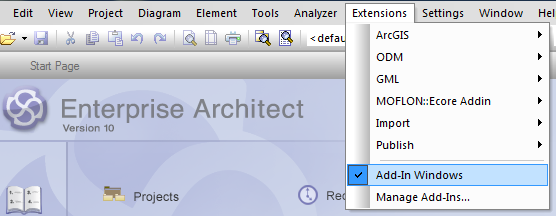
\includegraphics[width=1\textwidth]{../../org.moflon.doc.handbook.01_installation/2_simpleDemo/EADemo/images/ea_extensionMenu}
	\caption{Export from EA} 
	\label{ea:validate_dropdown} 
\end{figure}
%
\item
This tabbed control panel provides access to all of eMoflon's functionality.
This is where you can validate and export your complete project to Eclipse by pressing \menuPath{All} (\Cref{ea:controlPanel}).
%
\begin{figure}[htbp]
	\centering
  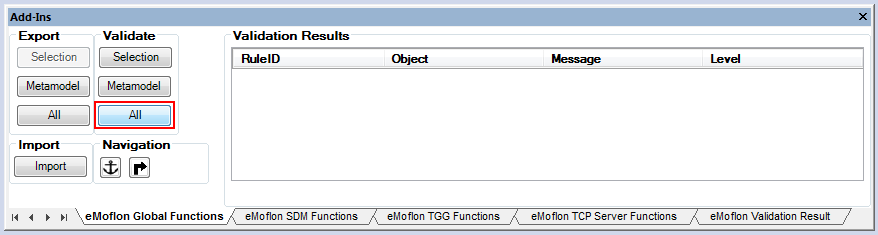
\includegraphics[width=0.9\textwidth]{../../org.moflon.doc.handbook.01_installation/2_simpleDemo/EADemo/images/ea_controlPanelValidateAll}
	\caption{eMoflon's control panel in EA} 
	\label{ea:controlPanel} 
\end{figure}
%
\item
Now try exploring the EA project browser!
Try to navigate to the packages, classes, and diagrams.
Don't worry if you don't understand that much---we'll get to explaining everything in a moment.
Just make sure not to change anything!

\item Switch back to Eclipse, choose your metamodel project, and press \shortcut{F5} to refresh. 
The export from EA places all required files in a hidden folder (\filename{.temp}) in the project.
A new, third project named \javaCode{org.moflon.demo.doublelinkedlist} is now being created.

\emph{Note:} If you refresh (for instance) \filename{.temp}, but nothing happens, then the Eclipse \emph{auto-build}\define{Auto-Build} is probably disabled.
Tick \menuPath{Project \menuSep Build Automatically} to re-enable it.
%
\item
Just wait until the workspace is fully built.
No error markers should be left---otherwise, double-check that auto-build is enabled.
%
\item
If you're ever worried about forgetting to refresh your workspace after exporting your specification from EA, or if you just don't want to bother with having to do this,
Eclipse does offer an option to do it for you automatically. To activate this, go to \menuPath{Window \menuSep Preferences \menuSep General \menuSep Workspace} and select \texttt{Refresh on access}.

\end{stepbystep}

\emph{Side note on the build process:}
The Eclipse auto-build framework normally cares for re-building your project whenever you modify your specification.
Still, there are situations in which you would like to build your project manually after a whole bunch of modifications, \eg, when your specification has grown very (very!) large.
To disable auto-build for a particular project, open the contained \menuPath{.project} file, locate either the \texttt{RepositoryBuilder} or the \texttt{IntegrationBuilder} and add a \texttt{<triggers>} element that contains the three build types \texttt{clean,full,incremental} (but not \texttt{auto}) such as in the following snippet.
\begin{lstlisting}[language=XML]
<buildCommand>
  <name>
    org.moflon.ide.core.runtime.builders.IntegrationBuilder
  </name>
  <triggers>clean,full,incremental</triggers> <!-- Add this line -->
  <arguments></arguments>
</buildCommand>
\end{lstlisting}
If auto-build is disabled for a particular project, this project is labeled with \enquote{[auto-build]} (\Cref{ea:noAutoBuild}).
%
\begin{figure}[htbp]
    \centering
    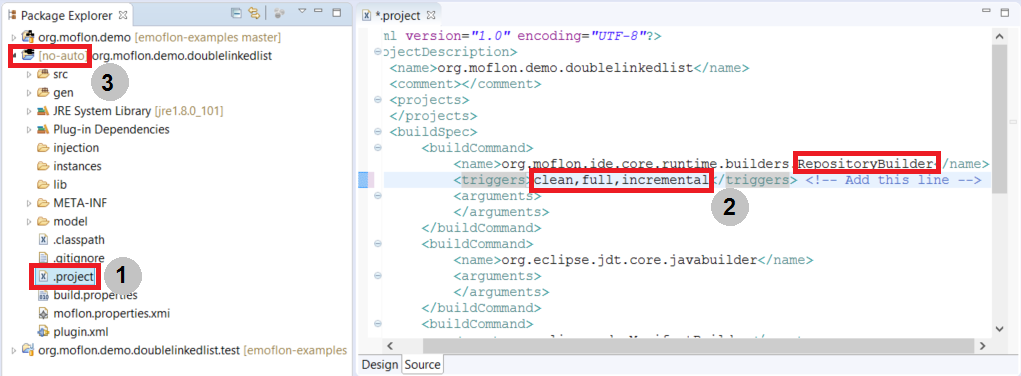
\includegraphics[width=\textwidth]{../../org.moflon.doc.handbook.01_installation/2_simpleDemo/EADemo/images/ea_noAutoBuild}
    \caption{Disabling auto-build for \texttt{org.moflon.demo.doublelinkedlist}} 
    \label{ea:noAutoBuild} 
\end{figure}
To facilitate triggering a manual build in situations where auto-build is switched off for one, several or even all projects, you may use the \enquote{eMoflon hammers}:
\begin{itemize}[*]
    \item
    The \emph{black hammer} \eMoflonFullBuildIcon triggers a full build (regardless of the changes since the last build).
    Alternatively, you may use the shortcut \linebreak \shortcut{Alt+Shift+E,B}.\footnote{First press \entity{Alt+Shift+E}, release, and press \entity{B}}
    By the way, most eMoflon shortcuts start with \linebreak\shortcut{Alt+Shift+E}.
    \item 
    The \emph{green hammer} \eMoflonIncrementalBuildIcon triggers an incremental build.
    Alternatively, you may use the shortcut \shortcut{Alt+Shift+E,D}.
\end{itemize}